% vim: set tw=78 tabstop=4 shiftwidth=4 aw ai:

\chapter{Designing an Improved Multiparty Protocol in the Linux Kernel}
\label{chapter:multiparty}

\todo{BitTorrent limitations, TCP vs. UDP, LEDBAT, P2P streaming, uTP,
uTorrent}

\section{The swift Multiparty Protocol}
\label{sec:multiparty:swift}

The \textit{swift} protocol is a generic multiparty transport protocol. Its
mission is to disseminate content among a swarm of peers. Basically, it
answers one and only one request: \textit{'Here is a hash! Give me data for
it!'}. Such entities as storage, servers and connections are abstracted and
are virtually invisible at the API layer. Given a hash, the data is received
from whatever source available and data integrity is checked cryptographically
with Merkle hash trees.

\todo{current implementation, TUDelft, Victor Grishcenko}

If you need some data it is somewhat faster and/or cheaper downloading it from
a nearby well-provisioned replica, but on the other hand, this process
requires that multiple parties (e.g. consumers, the data sources, CDN
sites, mirrors, peers) have to be coordinate. As the Internet
content is in a continuous increasing nowadays, the overhead of peer/replica
coordination becomes higher then the mass of the download itself. Thus, the
niche for multiparty transfers expands. Still, current, relevant technologies
are tightly coupled to a single use case or even infrastructure of a
particular corporation. These are the reasons of the \textit{swift} protocol
appearance with its primary goal to act as a generic content-centric
multiparty transport protocol that allows seamless, effortless data
dissemination on the big cloud represented by the Internet.

Most features of the \textit{swift} protocol are defined by its function as a
content-centric multiparty transport protocol. A significant difference
between \textit{swift} and the TCP protocol is that TCP possesses no
information regarding what data it is dealing with, as the data is passed from
the user-space, while the \textit{swift} protocol has data fixed in advance
and many peers participate in distributing the same data. Because of this and
the fact that for \textit{swift} the order of delivery is of little importance
and unreliability is naturally compensated for by redundancy, it entirely
drops TCP's abstraction of sequential reliable data stream delivery. For
example, out-of-order data could still be saved and the same piece of data
might always be received from another peer.

Being implemented over UDP, the protocol does its best to make every datagram
self-contained so each datagram could be processed separately and a loss of
one datagram must not disrupt the flow. Thus, a datagram carries zero or more
messages, and neither messages nor message interdependencies should span over
multiple datagrams.

The verification of data pieces is realize using Merkle hash
trees~\cite{merkle}, integrated as an extension in
BitTorrent\footnote{http://bittorrent.org/beps/bep\_0030.html}. That means
that all hashes necessary for verifying data integrity needs to be put into
the same datagram as the data. For both use cases, streaming and downloading,
an unified  integrity checking scheme that works down to the level of a single
datagram is developed. As a general rule, the sender should append to the data
some meta-data represented by the necessary hashes for the data verification.
While some optimistic optimizations are definitely possible, the receiver
should drop data if it is impossible to verify it. Before sending a packet of
data to the receiver, the sender inspects the receiver's previous
acknowledgments to derive which hashes the receiver already has for sure.

The data is acknowledged in terms of binary intervals, with the base interval
of 1KB "packet". As a result, every single packet is acknowledged logarithmic
number of times. This mechanism provides some necessary redundancy of the
acknowledgements and sufficiently compensates the unreliability of the
datagrams.

The only function of TCP that is also critical for \textit{swift} is the
congestion control. To facilitate delay-based congestion control an
acknowledgment contains besides the dimension of the file received from its
addressee a timestamp.

Our main objective is to integrate \textit{swift} as a transport protocol in
the Linux kernel networking stack. This will provide notable performance
improvement regarding data transfer. We intend to do this with minimal
intrusion effect in the Linux kernel and also to change as little as possible
the current \textit{swift} implementation. Another goal is to provide a
transparent API between the kernel and the user space. A developer will use a
socket-like interface when building an application on top of the
\textit{swift} protocol. In order to achieve this goal we have implemented an
intermediary step. We have simulated the kernel part in the user-space using
raw sockets. This has the advantage of providing means to have modular
functionality tests.

\todo{binmaps}
\todo{stadardization}

\section{Designing a Multiparty Protocol}
\label{sec:multiparty:design}

\todo{based on swift}
\todo{decisions: user-space, kernel-space}
\todo{phases: preliminary, raw sockets}
\todo{possibilities: socket interface, netlink sockets, device interface}
\todo{compatibility with socket interface}

\section{Preliminary Work}
\label{sec:multiparty:preliminary-work}

While designing our system, we have tackled a few different ideas, each with
its strengths and weaknesees. We present now some of those preliminary ideas
that lead to the our current desing choice.

The first approach we thought of was to include all of the swift protocol into
the kernel space. This approach had the advantage of simplicity and would have
implied minimal architectural changes. The current user space implementation
could have been ported to a kernel module.

Though simple, this approach could not be implemented because of the
restriction of memory size in the kernel.  For the integrity check the swift
protocol relies on Merkle hash tree. Keeping this tree in the kernel space
memory is not scalable. The Internet content is too large to be stored in
kernel. Even if the tree retains only hashes of the data disseminated, the
space is insufficient.

\begin{figure}
  \centering
  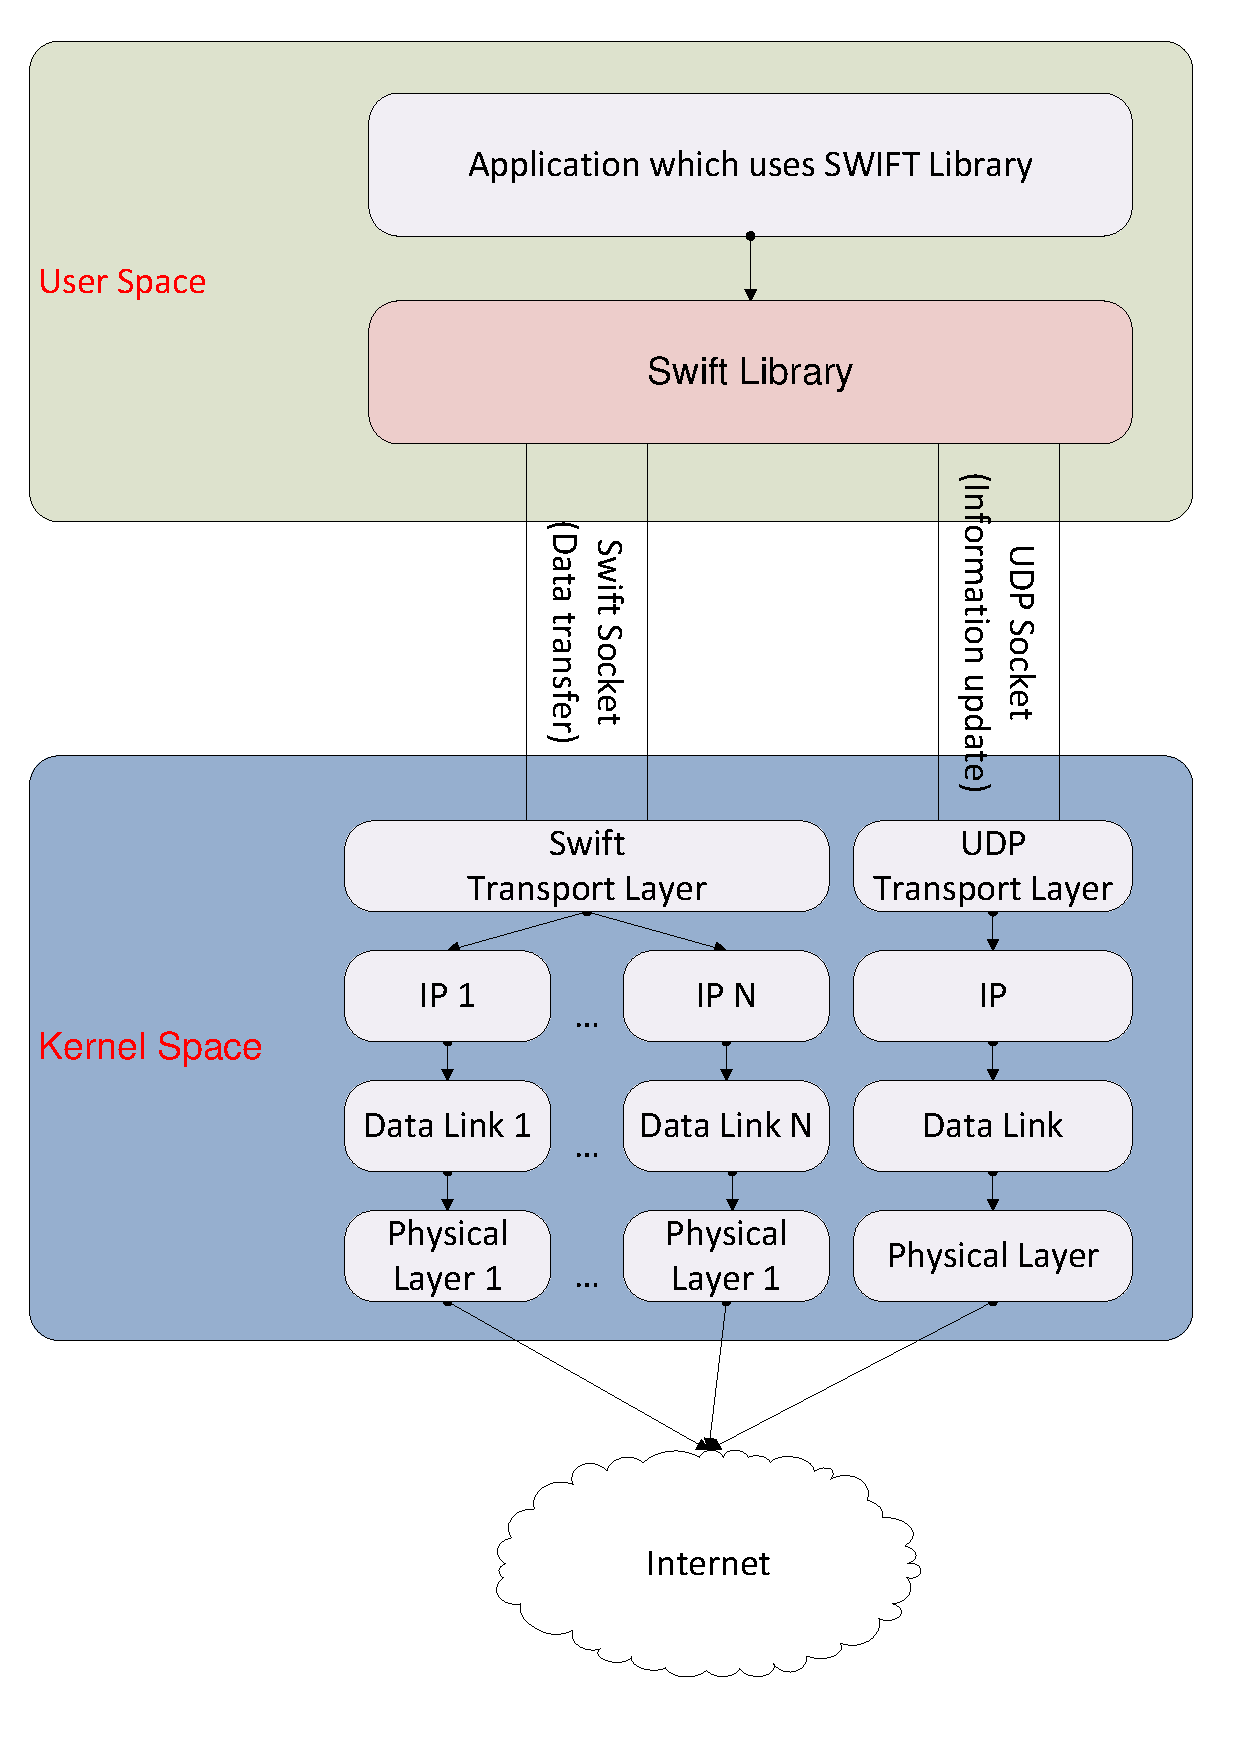
\includegraphics[width=0.4\textwidth]{src/img/multiparty/preliminary-architecture}
  \caption{Preliminary Architecture}
  \label{fig:multiparty:preliminary-architecture}
\end{figure}

The second approach of the swift implementation is represented in the
Figure~\ref{fig:multiparty:preliminary-architecture}. The swift transport
should have been a new kernel interface allowing the creation of specialized
swift sockets. It should have implemented the multiparty protocol allowing
piece transport to/from other hosts in a peer-to-peer fashion.

That implementation should have had specialized "request queues", metadata
queues, to/from user space. Specialized system call API should have allowed
user space applications to interact with the above mentioned queues and, thus,
with the multiparty transport protocol implementation.

Innate differences from a classical one-to-one communication such as UDP or
TCP means the system call API shouldn't have followed the classical
send/receive paradigm. In order to compensate this and to provide a rather
"friendly" interface to user space applications, a library was designed that
to provide a simpler interface. Peer and piece discovery should have been the
responsibility of the user space application. The SWIFT Library may also
provide wrappers over a UDP-based channel for discovery.

Merkle hashes should have stored and computed in user space. This approach
couldn't be implemented because of the restriction of the library
implementations (e.g. a users application design would be more restrictive).
Moreover the kernel implementation should have been like an UDP which support
multicast transfer.

The third approach of the swift implementation was to detach the transport
layer from the original swift implementation and to manage it. When we started
to implement this we found a lot of inconvenience like our code duplicate a
lot of application code, we cannot implement the discovery protocol, and again
our kernel implementation should have been like a multicast-UDP.

This approach also couldn't be implemented because of the complexity of the
transport layer management, moreover we didn't find strengths to confirm that
our implementation could be better than original implementation.

\section{Raw Socket Wrapper Implementation}
\label{sec:multiparty:raw-socket}

\todo{why new architecture}

\subsection{Architecture}

In this section we present our current architectural design along with the
motivation of choices. We are also going to detail our protocol and the packet
structure used.

In figure Figure~\ref{fig:multiparty:architecture-overview} we see the main
conceptual modules: Application module, wrapper library, peer discovery
overlay and the swift transport protocol layer.

\begin{figure}
  \centering
  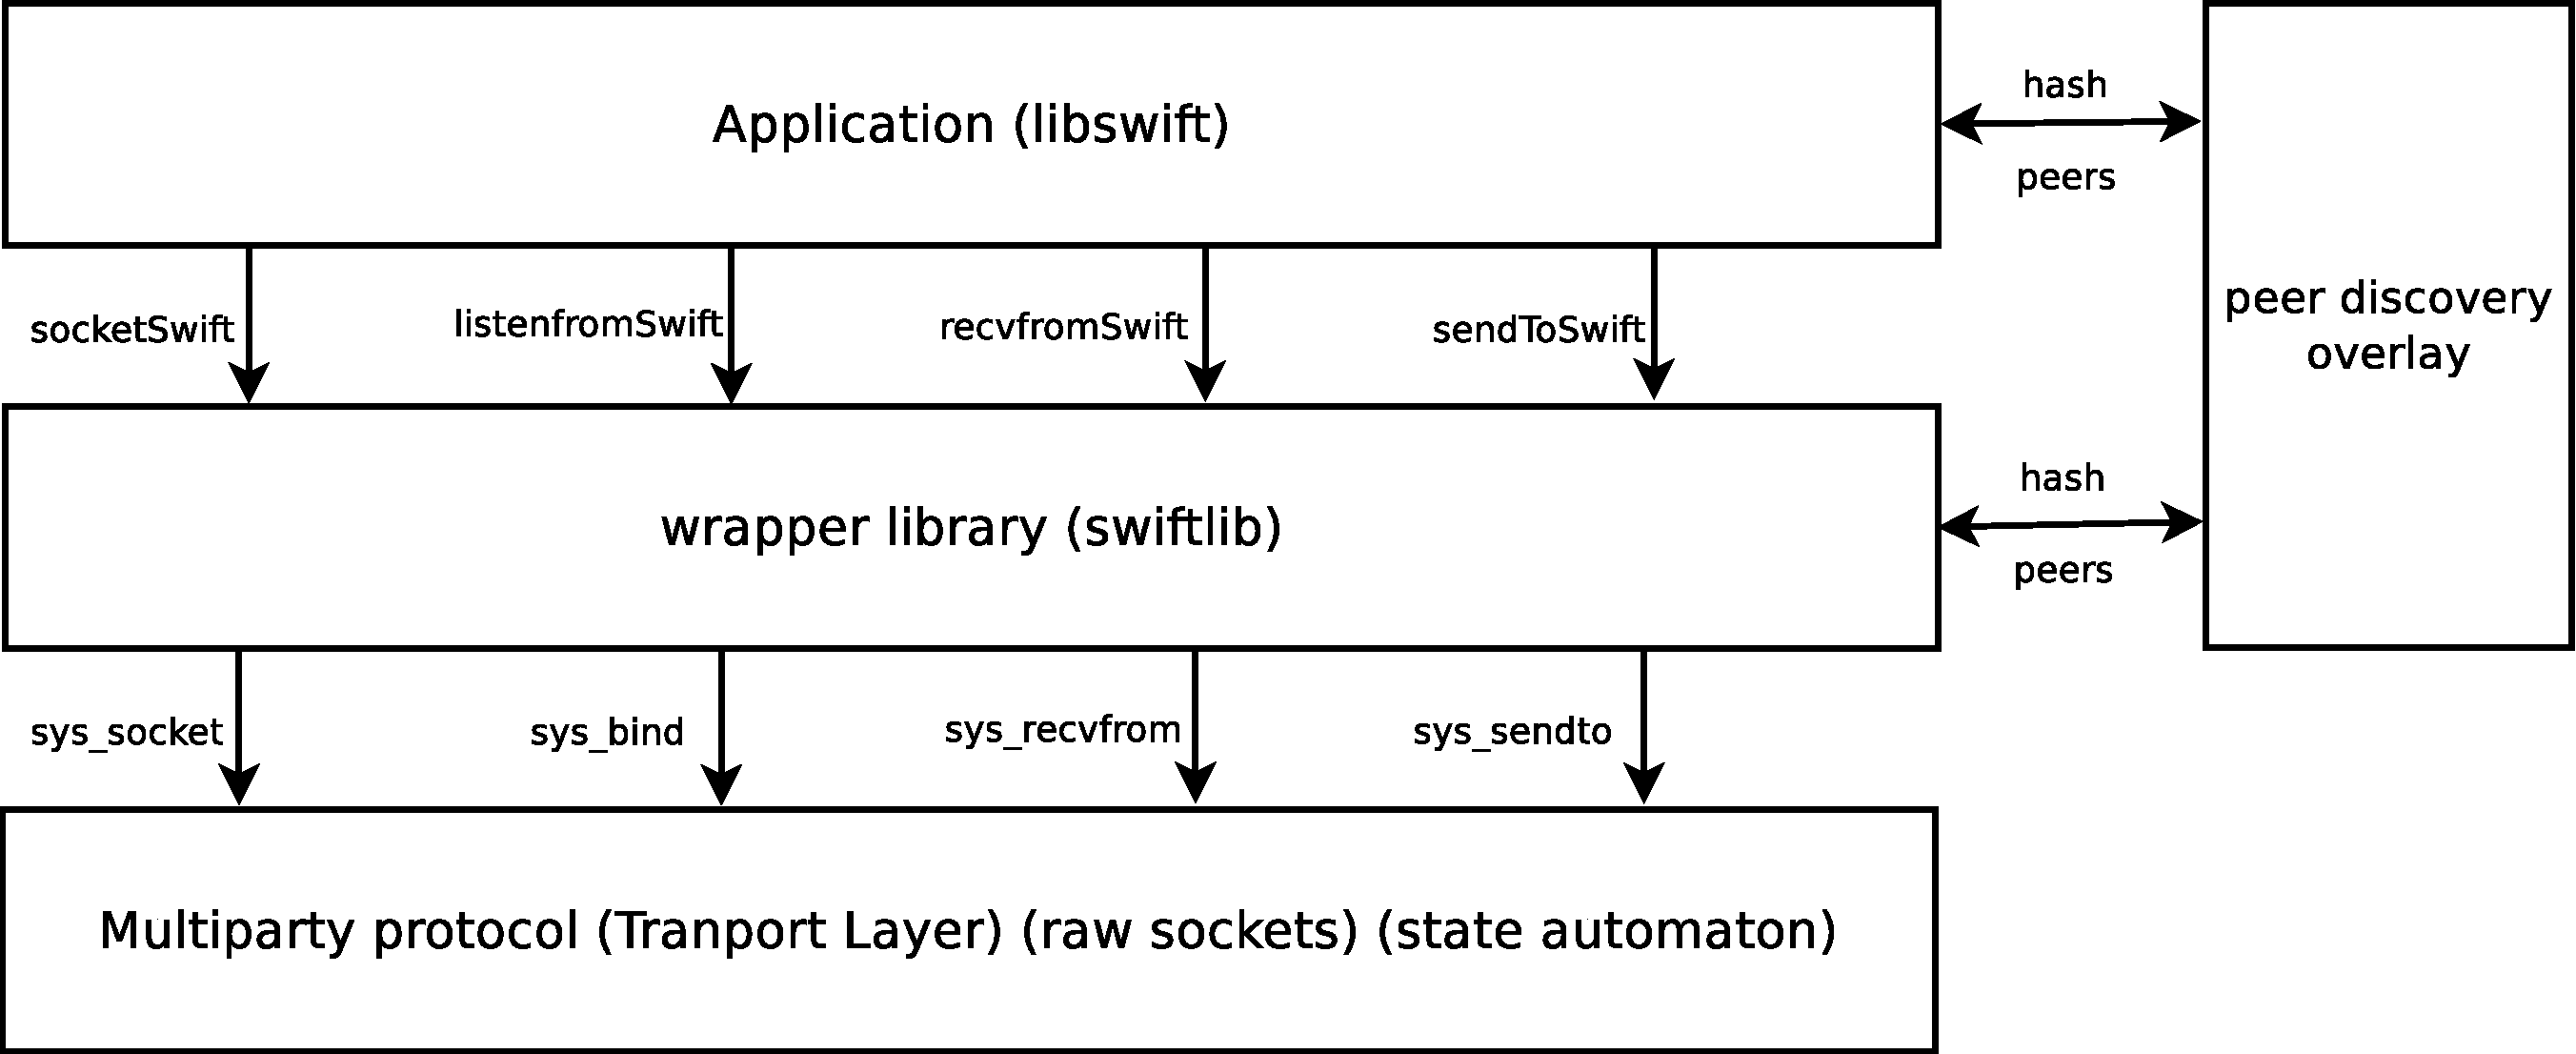
\includegraphics[width=0.4\textwidth]{src/img/multiparty/architecture-overview}
  \caption{Overview Architecture}
  \label{fig:multiparty:architecture-overview}
\end{figure}

The Application module represents the remaining part of the old swift
implementation. This is the part that remains in user space and contains the
file management and hash management features. 

The wrapper library module defines a socket-like API for the user space
applications. An regular program will use those calls instead of the normal
socket ones to use the multiparty sockets. For the moment those calls are
simulated system calls that initially are resolved with the socket raw
implementation (still in user space). In the future this wrapper library
will represent entry points into the kernel.

The peer discovery overlay will remain unchanged. It is still going to work
based on UDP sockets and link the same levels in the swift implementation as
before. The peer discover will be part of the application implementation and
it will be at the developer choice how to implement and how to manage it.

The multiparty protocol is implemented for now at user space level by a raw
socket layer to validate our architecture.  This has the advantage of
simulating the real design modularization but also permit an easier debugging
and testing procedure of the integration. In the next step this part will be
represented by a kernel patch that will communicate through custom made system
calls with the wrapper library. This two phases are described in
Figure~\ref{fig:multiparty:detailed-architecture}.

\begin{figure}
  \centering
  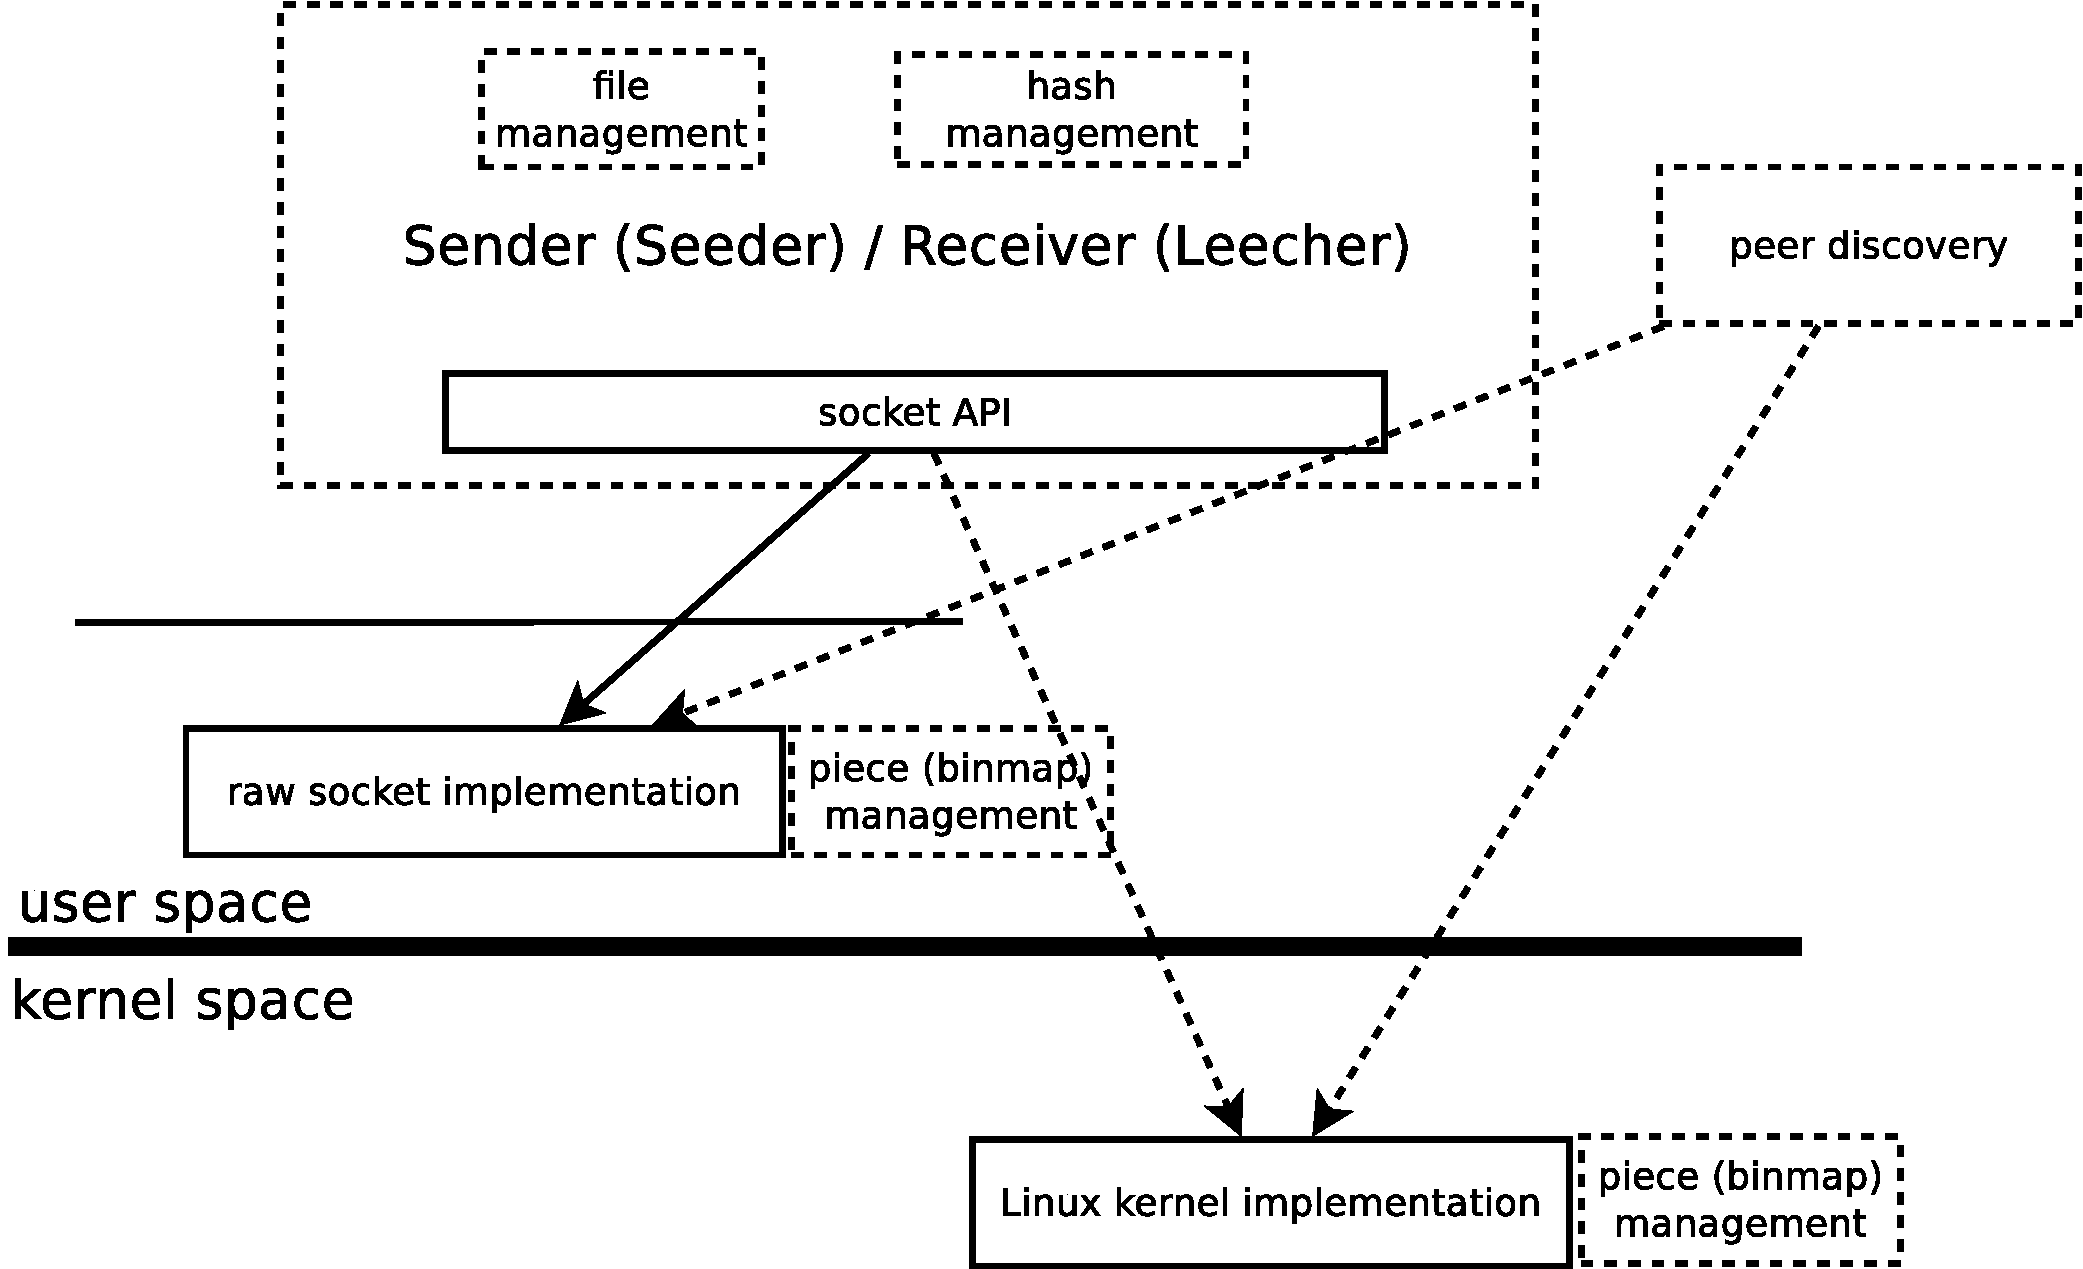
\includegraphics[width=0.4\textwidth]{src/img/multiparty/detailed-architecture}
  \caption{Detailed Architecture}
  \label{fig:multiparty:detailed-architecture}
\end{figure}

A socket is one of the most fundamental technologies of computer networking.
Sockets allow applications to communicate using standard mechanisms built into
network hardware and operating systems.

Raw mode is basically there to allow you to bypass some of the way that your
computer handles TCP/IP. Rather than going through the normal layers of
encapsulation/decapsulation that the TCP/IP stack on the kernel does, you just
pass the packet to the application that needs it. No TCP/IP processing -- so
it's not a processed packet, it's a raw packet. The application that's using
the packet is now responsible for stripping off the headers, analyzing the
packet, all the stuff that the TCP/IP stack in the kernel normally does for
you.

Raw socket implementation will support all syscalls and it will be a copy of
our kernel implementation.  This implementation will have the same API and
behavior as the kernel implementation. Still, in the first implementation, a
swift socket will be available to act as only a seeder or a leecher,
explicitly one operation transmit data or receive data will be supported.

In the last implementation the swift protocol will be develop in kernel space,
and it will be accessible with a datagram socket that will support all socket
syscalls. It will intend to support both operations (receive / send) data over
only one socket.

\begin{figure}
  \centering
  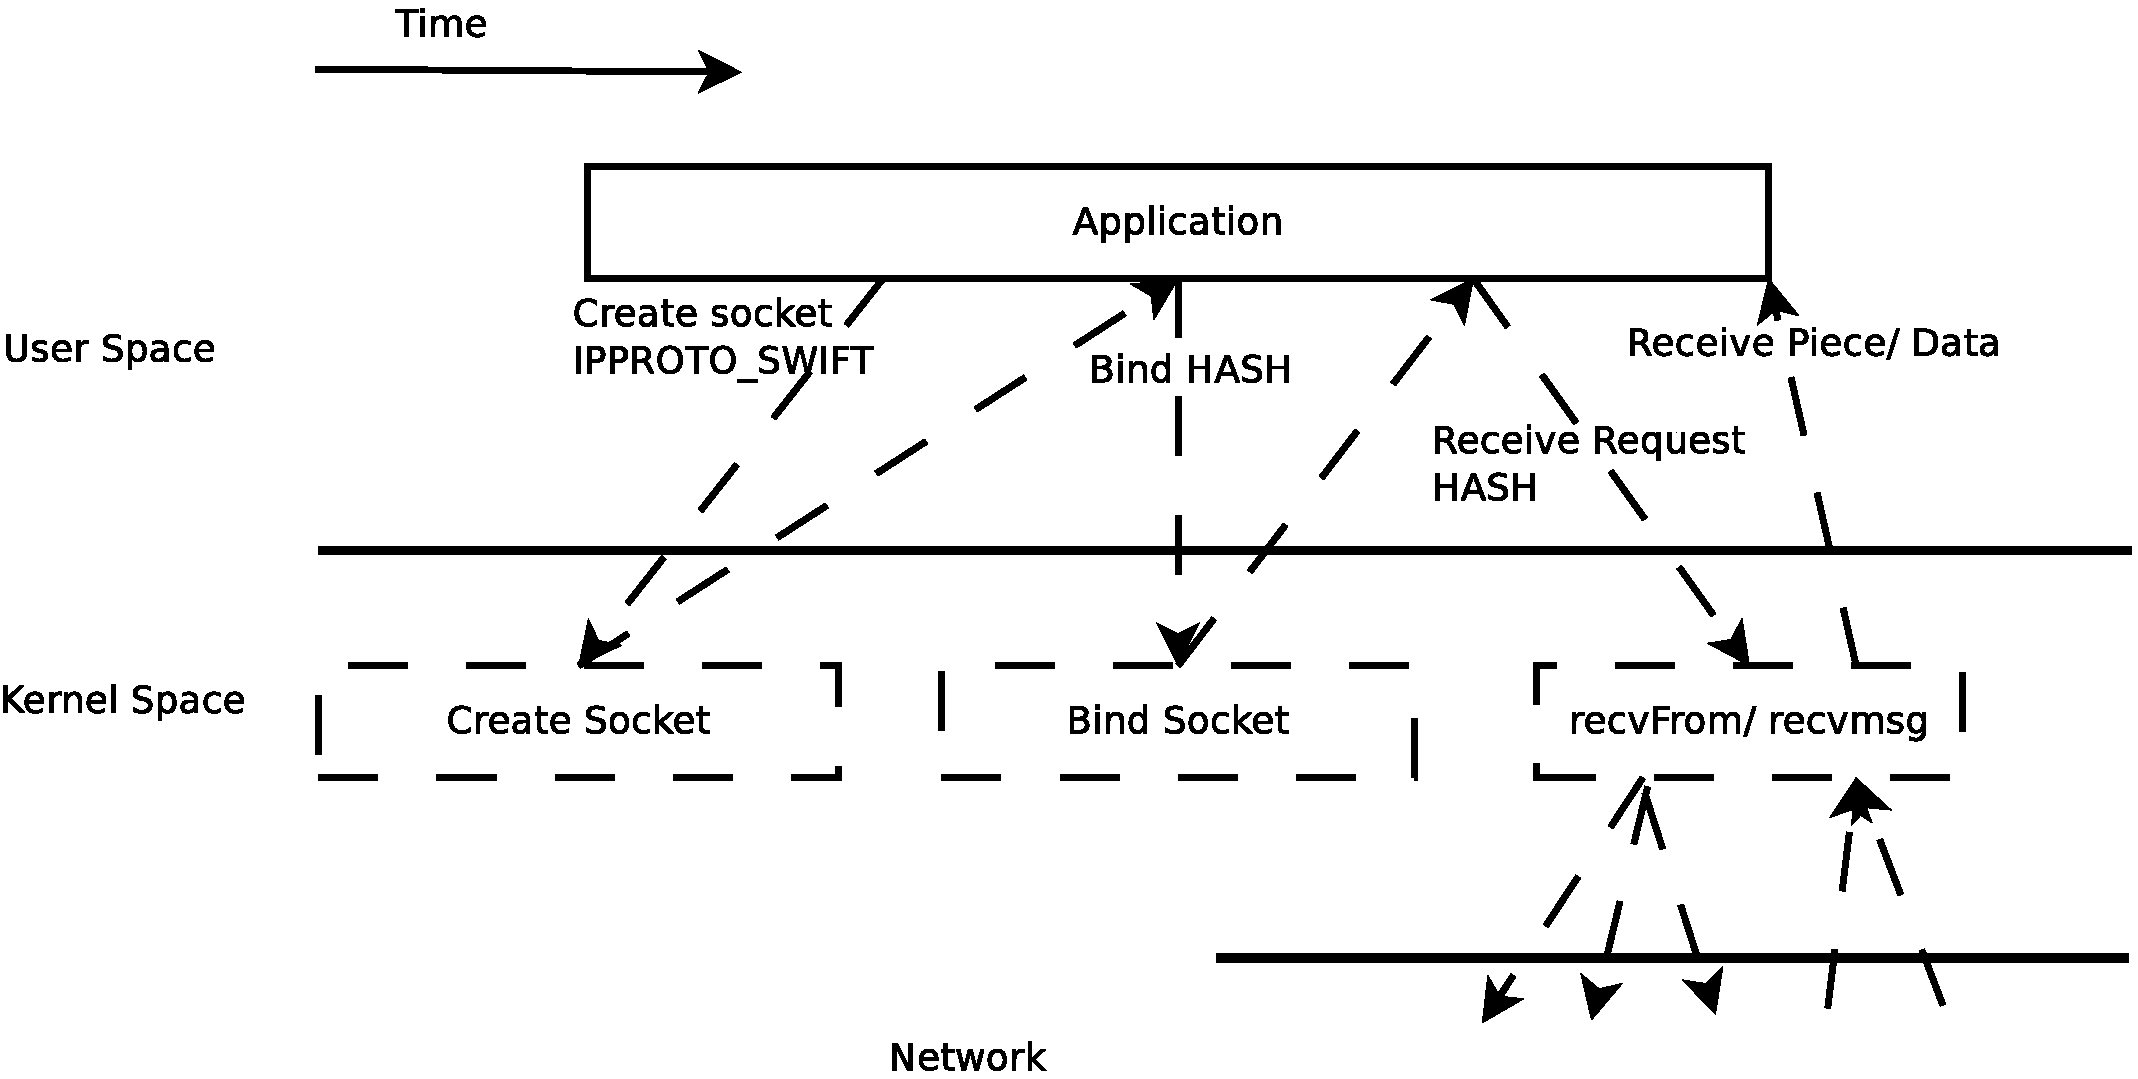
\includegraphics[width=0.55\textwidth]{src/img/multiparty/multiparty-recvmsg}
  \caption{Receiver Conceptual Model}
  \label{fig:multiparty:multiparty-recvmsg}
\end{figure}

Figure~\ref{fig:multiparty:multiparty-recvmsg} presents the conceptual model
of the Leecher. The Leecher is the one that wants to receive a data. In order
to do this it must connect to the multiparty protocol by creating and binding
to a multiparty socket. When it binds to a socket, it uses the hash as a
parameter to find a connection with a peer that has the respective file. This
discovery is done the peer discovery overlay. The Leecher then waits for
packets from the seeders.

\begin{figure}
  \centering
  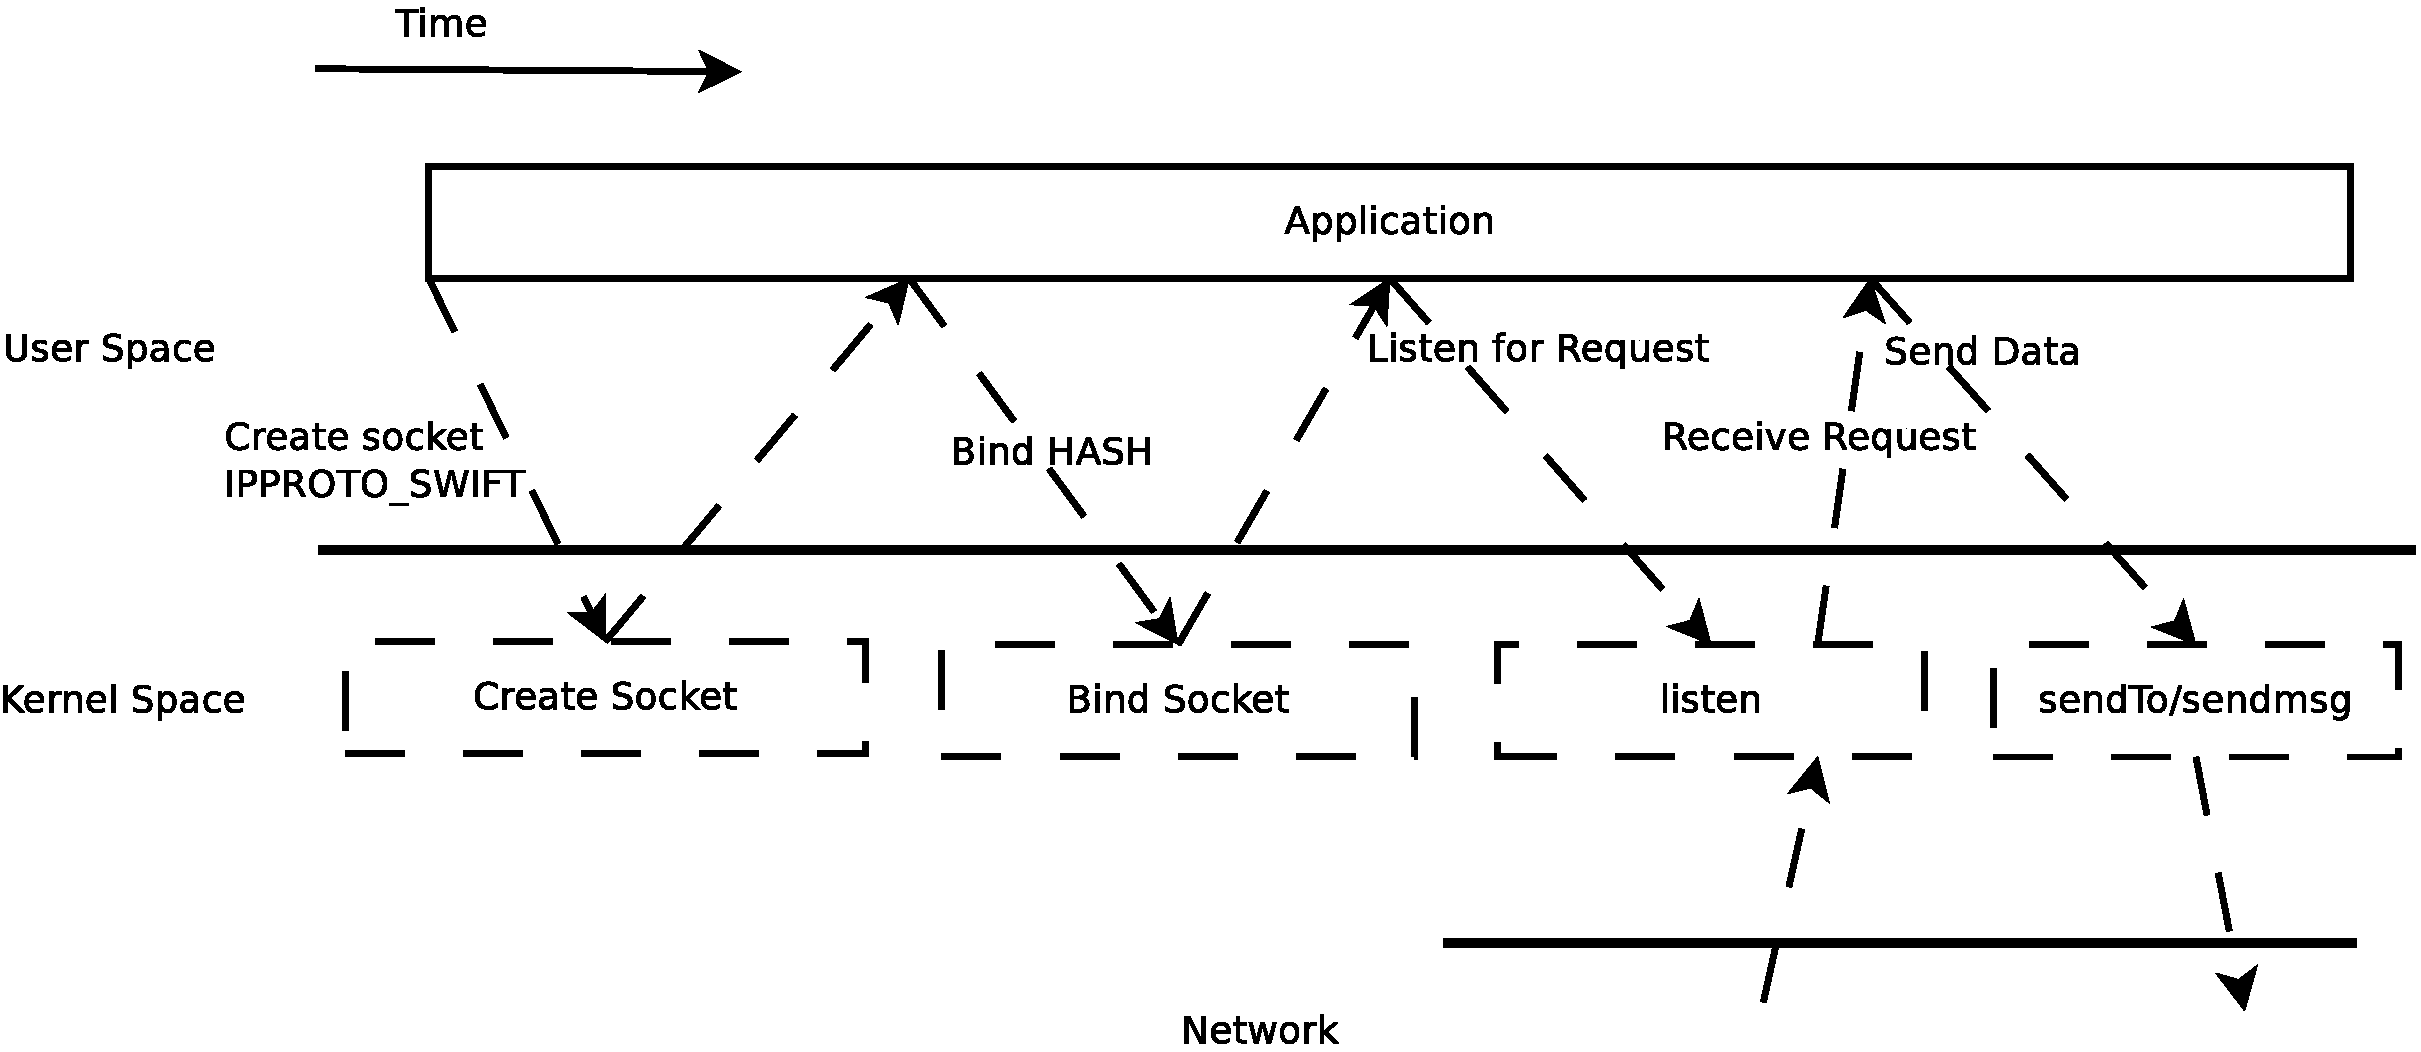
\includegraphics[width=0.55\textwidth]{src/img/multiparty/multiparty-sendmsg}
  \caption{Sender Conceptual Model}
  \label{fig:multiparty:multiparty-sendmsg}
\end{figure}

Figure~\ref{fig:multiparty:multiparty-sendmsg} presents the conceptual model
of the Seeder. The Seeder is the one that serves data to other Leechers. In
order to do this it must connect to the multiparty protocol by creating,
binding and listening to a mutliparty socket. When binding the Seeder
practically uses the hash as a parameter. This means that for every file
hashed there will be a socket on which the seeder can receive and serve
requests. The Seeder then waits for requests and sends data packets as
requested.

\subsection{Testing}

The  protocol is a generic multiparty transport protocol. Its mission is to
disseminate content among a swarm of peers.  Given a hash, the data is
received from whatever source available and data integrity is checked
cryptographically with Merkle hash trees. 

Our main focus when modifying the swift implementation is to have an impact on
time performance. With a communication protocol the greatest latency is
usually generated by waiting for the results from the network. The multiparty
communication model already takes care of this, so the next best thing is to
enhance the application time. We are doing this by decreasing the time
penalties due to context switches between user space and kernel space. The
main idea is to reduce the number of system calls made from user space into
the kernel. This implicitly reduces the number of preemption moments.

Firstly, we have implemented a test suite for every socket system call, which
test all possible cases.  This unit tests are made to ensure the code quality,
and to validate if the system call respond in the same mode as other similar
system call.

Secondly, we have implemented a functional tests to validate a simple
workflow. For this purpose we have a sender that acts as the seeder and a
receiver which have the leecher role. We transfer a small file between this
entities.

Also we will implement performance tests that will validate our design and
implementation. This tests will compare the number of system calls for both
implementation (original implementation and our implementation).

\section{Kernel Framework for Multiparty Protocol Implementation}
\label{sec:multiparty:kernel-framework}

The introduction of a multiparty protocol in the Linux kernel was a challenge,
because of its particularities versus common protocol implementations. A
multiparty transport protocol uses multiple points in a communication, unlink
a traditional communication protocol that allows a sender endpoint and a
receiver endpoint.

A traditional Tranport Layer protocol header uses a port to differentiate
between various processes that take part in a communication and use Network
Layer address information for host information. For a multiparty Transport
Layer protocol, the port information would be substituted by a file. While
traditional protocol use ``data'' (either streams -- TCP, or datagrams --
UDP), a multiparty protocol is concerned about sending and receiving parts of
a given file, which significantly alters its design.

Currently, the swift protocol~\cite{TODO} that forms the basis of the
current design is implemented in user space, using UDP sockets. There is no
need for TCP, as ordered delivery offered by TCP is of no importance to swift.
Packets may be received out of of order and the same piece of information may
be received multiple times from different peers. Redundancy is important to
swift: the first arriving piece is added to the ``stream'' while the rest are
discarded.

The main feature of the swift protocol is that it's content-centric, unlike
TCP that possesses no knowledge of the transported data. Data possesses
meaning for swift.

Checking pieces that are received through swift is accomplished through the
use of Merkle hash trees~\cite{TODO}. This means that all information
regarding integrity checking is already placed in the same data packet.

\todo{focus on it being a module}

\subsection{Tranport Protocol Implementation on the Linux Kernel}

In order to implement o transport protocol in the Linux kernel, several design
phases must be established:

\begin{itemize}
  \item Defining \texttt{IPPROTO\_\$\$}. This macro will identify the
  transport protocol. This will be subsequently used for creating a transport
  protocol socket.
  \item Defining a transport header. The framework we used defined two 8 bit
  ports, a source port and a destination port and a 16 bit lenght field. The
  latter field is the data length, including the tranport protocol header.
\end{itemize}

After the above have been completed, several data structures have to be
defined, as mentioned below.

A data structure that defines the new coket type. This is where we must save
information regarding the socket state, such as the destination or the source
port.
\begin{verbatim}
struct swift_sock {
    struct inet_sock sock;
    /* swift socket speciffic data */
    uint8_t src;
    uint8_t dst;
};
\end{verbatim}

The protocol definition, used by the socket, including its name and size are
defined in a \texttt{struct proto} structure.
\begin{verbatim}
static struct proto swift_prot = {
    .obj_size = sizeof(struct swift_sock),
    .owner = THIS_MODULE,
    .name = "SWIFT",
};
\end{verbatim}

The most important structure to be defined describses the operations that are
supported by a socket of a given type. For a datagram sending socket, the
implementation of \texttt{release}, \texttt{connect}, \texttt{sendmsg} and
\texttt{recvmsg} functions is sufficient.
\begin{verbatim}
static const struct proto_ops swift_ops = {
    .family = PF_INET,
    .owner = THIS_MODULE,
    .release = swift_release,
    .bind = swift_bind,
    .connect = swift_connect,
    .socketpair = sock_no_socketpair,
    .accept = sock_no_accept,
    .getname = sock_no_getname,
    .poll = datagram_poll,
    .ioctl = sock_no_ioctl,
    .listen = sock_no_listen,
    .shutdown = sock_no_shutdown,
    .setsockopt = sock_no_setsockopt,
    .getsockopt = sock_no_getsockopt,
    .sendmsg = swift_sendmsg,
    .recvmsg = swift_recvmsg,
    .mmap = sock_no_mmap,
    .sendpage = sock_no_sendpage,
};
\end{verbatim}

The new packtets header are setup in the \texttt{net\_protocol} header. New
packets that are received directly from the network will fill the
\texttt{protocol} field in the IP header with the value of the implemented
Transport Level protocol.
\begin{verbatim}
static const struct net_protocol swift_protocol = {
    .handler = swift_rcv,
    .no_policy = 1,
    .netns_ok = 1,
};
\end{verbatim}

A final data structure has to connect the new protocol to the operations on
the its socket. This structure uses two pointers to the \texttt{struct proto}
and \texttt{struct proto\_ops} data structures:
\begin{verbatim}
static struct inet_protosw swift_protosw = {
    .type = SOCK_DGRAM,
    .protocol = IPPROTO_SWIFT,
    .prot = &swift_prot,
    .ops = &swift_ops,
    .no_check = 0,
};
\end{verbatim}

As soon as the above structures are defined, the protocol defined will be
added to the kernel. The sequence of operations used to establish this step is
described below.

\begin{verbatim}
proto_register(&swift_prot, 1);
inet_add_protocol(&swift_protocol, IPPROTO_SWIFT);
inet_register_protosw(&swift_protosw);
\end{verbatim}

Befor compiling and inserting the module in the kernel, several socket
operations functions have to be filled; for swift (a datagram based protocol),
this would mean \texttt{release}, \texttt{bind}, \texttt{connect},
\texttt{sendmsg} and \texttt{recvmsg}. A handler for packets received from the
network must also be implemented. At protocol level, one must keep a mapping
between a port and a socket, meaning that the socket is bound tot that port.

Each implemented socket operations functions fills different roles:

\begin{itemize}
  \item \texttt{release} is used fo freeing resources (most likely memory)
  used by the socket.
  \item \texttt{bind} checks the availability of the port and ties the socket
  to that port and a source IP address.
  \item \texttt{connect} maps the current socket to a destination port and IP
  address.
  \item \texttt{sendmsg} extracts the destination IP address and port,
  provided they were passed as arguments from user space. If they were not
  provided, the module checks whether the socket is connected (through a
  previous \texttt{connect} call), and, in case no socket is connected, error
  is returned.

  After establishing the receiving end (IP address and port), an
  \texttt{skb} structure is allocate, specifying the protocol header and the
  rest of the data. The swift header is filled, user space data are copied and
  the packet is routed. After the routing process, required data is copied and
  is queued for transmit using the \texttt{ip\_queue\_xmit} function call.

  \item \texttt{recvmsg} is responsible for the reverse operation of
  \texttt{sendmsg}. A datagram is read from the receiving queue through the
  use of the \texttt{skb\_recv\_datagram} call. Serveral integrity checks are
  employed, after which data is copied from the \texttt{skb} structure to user
  space.

  At the time, in case the sender address (IP address and port) has been
  requested (as used by the \texttt{recvmsg} and \texttt{recvfrom} socket API
  call), required information is filled in the user space buffer.

  In the end the \texttt{skb} structure is freed through the use of the
  \texttt{skb\_free\_datagram} call.

  \item The function passed as a handler in the \texttt{net\_protocol}
  structure is invoked when a packed is received. The protocol field in the
  packet IP header will be used to demultiplex the packet and call the
  required function.

  When the packet is received, several validations of this will take place.
  Subsequently, the destination port information will be extracted. A lookup
  operation returns the socked mapped to the destination port. The
  \texttt{skb->cb} field is initialized to information regarding the sender.
  Afterwards, the packed is added to the receive queue, through the use of
  \texttt{ip\_queue\_rcv\_skb}.
\end{itemize}

\subsection{Testing}

Unit testing has been employed for testing the protocol. Among those are a few
simple tests, to ensure basic functionality and then a set of new tests that
check error codes and protocol performance. Protocol performance is related to
ensuring scalability -- multiple simulateneous client connections.

Basic functional testing means the design and implementation of tests for each
function exposed by the protocol. That is, there is a given test for each of
\texttt{bind}, \texttt{connect}, \texttt{close}, \texttt{sendto},
\texttt{recvfrom}, \texttt{sendmsg}, \texttt{recvmsg}, \texttt{send} and
\texttt{recv}.

Negative testing, for unwanted/unwelcome situations is similarly accomplished:
each function exposed by the protocol is assigned a test. For example, the
\texttt{bind} system call will always check an error being returned for a
duplicate call using the same port. As is the case for the use of invalid IP
addresses or invalid port numbers. A series of such tests will be employed for
each functionality.

Performance testing is completed through the use of multiple protoocl sockets.
Data is sent from the socket is is checked against data arriving at the other
end; this actually means checking whether port and socket mapping is working
according to the specifications. Another measure of protocol performance is
the transfer speed on the newly created socket.

\section{Conclusion}
\label{sec:multiparty:conclusion}

The \textit{swift} protocol is a multiparty content-centric protocol that aims
to disseminate content among a swarm of peers. This chapter proposes an
approach for the optimization of the currently \textit{swift} protocol. The
integration of the communication in the kernel space as a multiparty transport
protocol that is solely responsible for getting the bits moving improves the
over all protocol performance. It ensures maximum efficiency of data transfer
by decreasing switches between user and kernel space and eliminating some
performance penalties due to context switches.

After we complete the implementation and the functional tests, we want to test
extensively our new features in a real environment. We plan to do stress tests
using a cluster. This tests will help us to make an overview about our
implementation and we could compare with the user-space implementation of the
\textit{swift} to determine exactly what performance we encountered. If the
results are satisfactory, we will continue to optimize our program and we will
add new features.

It will be very useful to have a real application on top of the \textit{swift}
protocol. If not, one solution would be to port an application strictly for
this task. This would give us the opportunity to extend and refine our
implementation, and also to extend the library API.

The multiparty protocol is planned to be implemented in the Linux kernel, by
adapting it to the framework described above. By bringing the protocol to the
kernel, its performance should increase due to the decrease in the number of
user space/kernel space swiches (as part of the decrease of system calls).

Currently the framework lacks a packet fragmentation mechanism. The current
implementation can't send on a socket data larger then the \textit{Maximum
Transfer Unit} (\textit{MTU}) (1500 bytes for Ethernet). A possible solution
is borrowing the fragmentation mechanism used by the UDP implementation.
